% =============================================================================
%  The Monetary-Financial-Fiscal Macromodel (MFFM) — Senior Management presentation
%  Template + palette adapted from docs/Global_estimation_of_nonlinear_DSGE_models
%  Compile with pdfLaTeX. Self-contained (figures/ holds the tool screenshots).
% =============================================================================
\documentclass[aspectratio=169,10pt]{beamer}
\usetheme{default}
\setbeamertemplate{navigation symbols}{}
\setbeamertemplate{itemize items}[triangle]

\usepackage{amsmath,amssymb,bm}
\usepackage{booktabs}
\usepackage{graphicx}
\usepackage{tikz}
\usetikzlibrary{arrows.meta,positioning,calc,shapes.geometric}
\emergencystretch=3em
\graphicspath{{figures/}}

% ---- palette + macros (from Farkas_CEF_slides.tex) ----
\definecolor{MadridBlue}{RGB}{28,54,99}
\definecolor{MadridBlue2}{RGB}{48,91,150}
\definecolor{Ink}{RGB}{35,35,35}
\definecolor{Muted}{RGB}{105,105,105}
\definecolor{LightGrey}{RGB}{244,245,247}
\definecolor{MidGrey}{RGB}{210,214,221}
\definecolor{SoftBlue}{RGB}{235,241,249}
\definecolor{SoftBlue2}{RGB}{224,233,246}
\definecolor{AccentRed}{RGB}{150,45,45}
\definecolor{CheckGreen}{RGB}{39,116,75}

\setbeamercolor{normal text}{fg=Ink,bg=white}
\setbeamercolor{frametitle}{fg=white,bg=MadridBlue}
\setbeamercolor{structure}{fg=MadridBlue}
\setbeamercolor{footline}{fg=Muted}
\setbeamerfont{frametitle}{series=\bfseries,size=\large}
\setbeamerfont{title}{series=\bfseries,size=\Large}
\setbeamerfont{footline}{size=\scriptsize}
\setbeamertemplate{frametitle}{%
  \nointerlineskip
  \begin{beamercolorbox}[wd=\paperwidth,sep=0.28cm,leftskip=0.16cm,rightskip=0.16cm plus1fil]{frametitle}%
    \strut\insertframetitle\strut%
  \end{beamercolorbox}%
}
\setbeamertemplate{footline}{%
  \hfill{\usebeamerfont{footline}\usebeamercolor[fg]{footline}\insertframenumber}\hspace{0.55em}\vspace{0.45em}
}
\newcommand{\key}[1]{\textbf{\textcolor{MadridBlue}{#1}}}
\newcommand{\gap}[1]{\textcolor{AccentRed}{#1}}
\newcommand{\todo}[1]{{\footnotesize\color{AccentRed}\itshape[#1]}}
\newcommand{\takeaway}[2]{%
  \par\vspace{0.4em}%
  {\setlength{\fboxsep}{0.62em}\setlength{\fboxrule}{0.6pt}%
   \noindent\fcolorbox{MadridBlue}{SoftBlue}{%
   \parbox{\dimexpr\linewidth-2\fboxsep-2\fboxrule\relax}{\textbf{\color{MadridBlue}#1: \\}\,#2}}\par}%
}
\newcommand{\plus}{\item[\textcolor{CheckGreen}{\textbf{+}}]}
\newcommand{\fignote}[1]{\par\vspace{0.15em}{\scriptsize\color{Muted}#1}}
\newcommand{\fig}[2]{\IfFileExists{figures/#2.png}{\includegraphics[width=#1]{#2}}{\fbox{\parbox[c][3cm][c]{#1}{\centering\color{Muted}\small [figure: #2]\\ \tiny to be captured}}}}
% \figmask{width}{name} — the figure MASKED to a soft rounded rectangle with a hairline border, for a
% designed, "card"-like look (less chrome, more focus).
\newcommand{\figmask}[2]{%
  \IfFileExists{figures/#2.png}{%
  \begin{tikzpicture}
    \node[inner sep=0pt] (im) {\phantom{\includegraphics[width=#1]{#2}}};
    \begin{scope}
      \clip[rounded corners=6pt] (im.south west) rectangle (im.north east);
      \node[inner sep=0pt] at (im.center) {\includegraphics[width=#1]{#2}};
    \end{scope}
    \draw[rounded corners=6pt, draw=MidGrey, line width=0.7pt] (im.south west) rectangle (im.north east);
  \end{tikzpicture}%
  }{\fbox{\parbox[c][2.6cm][c]{#1}{\centering\color{Muted}\small [#2]}}}}

% flow-box style for the pipeline strip / section marker
\tikzset{
  stage/.style={rounded corners=3pt, draw=MadridBlue, line width=0.7pt, fill=SoftBlue,
    text=Ink, align=center, inner sep=4pt, minimum height=0.95cm, font=\scriptsize, text width=2.15cm},
  stageon/.style={stage, fill=MadridBlue, text=white},
  flowarr/.style={-{Stealth[length=2mm]}, draw=MadridBlue2, line width=0.9pt},
}
% Compact "you-are-here" strip: #1 = index (1..5) of the highlighted stage.
\newcommand{\roadmap}[1]{%
\begin{center}\begin{tikzpicture}[every node/.style={font=\tiny}]
  \foreach \i/\lab [count=\c] in {1/Baseline,2/Conditioning,3/Global solve,4/Extensions,5/Conclusion}{%
    \pgfmathparse{\i==#1 ? "stageon" : "stage"}\edef\st{\pgfmathresult}%
    \ifnum\i=1 \node[\st,text width=1.7cm,minimum height=0.5cm] (n\i) {\lab};%
    \else \node[\st,text width=1.7cm,minimum height=0.5cm,right=0.35cm of n\the\numexpr\i-1\relax] (n\i) {\lab}; \draw[flowarr] (n\the\numexpr\i-1\relax) -- (n\i);\fi}
\end{tikzpicture}\end{center}}

\title[MFFM]{The Monetary--Financial--Fiscal Model (MFFM)}
\author[M. Farkas]{M\'aty\'as Farkas}
\institute[IMF]{International Monetary Fund}
\date{Senior Management briefing}

\begin{document}

% =============================================================================
% 1. TITLE
% =============================================================================
\begin{frame}
  \vspace{1.7em}
  {\usebeamerfont{title}\color{MadridBlue}The Monetary--Financial--Fiscal Model (MFFM)\par}
  \vspace{0.55em}
  {\color{MadridBlue}\rule{0.40\linewidth}{1.1pt}}\par
  \vspace{0.65em}
  {\large\color{Ink}A global projection and scenario tool ---\\
   one coherent ``what-if'' for 50 economies, and its policy implications.\par}
  \vfill
  {\normalsize\color{Ink}M\'aty\'as Farkas\par}
  \vspace{0.15em}
  {\small\color{Muted}International Monetary Fund\par}
  \vspace{0.9em}
  {\small\color{Muted}Senior Management briefing \quad\textbullet\quad \todo{date / venue}\par}
  \vspace{1.4em}
  {\scriptsize\color{Muted}Views expressed are my own and do not necessarily represent the IMF.}
\end{frame}

% =============================================================================
% 2. MOTIVATION  (GMF text to be added by MF / Jesper)
% =============================================================================
\begin{frame}{Why now: the next generation of the Fund's global macro-financial model}
\vspace{0.3em}
\begin{columns}[T,onlytextwidth]
\begin{column}{0.48\textwidth}
  {\small\bfseries\color{MadridBlue} Today: the GMF (Vitek)}
  \begin{itemize}\setlength\itemsep{3pt}\small
    \item Served the Fund well as a global macro-financial workhorse.
    \item[\textcolor{AccentRed}{\textbf{--}}] \gap{Not updated in estimation} --- \todo{MF/Jesper: specifics}
    \item[\textcolor{AccentRed}{\textbf{--}}] \gap{Missing FSAP / Article~IV features} --- \todo{MF/Jesper: list the needs}
    \item[\textcolor{AccentRed}{\textbf{--}}] \todo{MF/Jesper: any further gaps}
  \end{itemize}
\end{column}
\begin{column}{0.48\textwidth}
  {\small\bfseries\color{MadridBlue} What surveillance now needs}
  \begin{itemize}\setlength\itemsep{3pt}\small
    \plus Current estimates, refreshed each cycle.
    \plus Fast, transparent scenarios for FSAP \& Article~IV.
    \plus Genuine cross-border transmission, not country-by-country.
    \plus \todo{MF/Jesper: the specific FSAP/AIV features}
  \end{itemize}
\end{column}
\end{columns}
\takeaway{The case}{\todo{MF/Jesper: one-line motivation --- e.g.\ ``The MFFM supersedes the GMF: re-estimated, scenario-ready, and built for FSAP--Article~IV work.''}}
\end{frame}

% =============================================================================
% 3. ADVANTAGES / WHAT'S NEW
% =============================================================================
\begin{frame}{What the MFFM adds --- five things it does that a static model cannot}
\vspace{0.5em}
\begin{itemize}\setlength\itemsep{5pt}
  \plus \key{Re-estimated and current.} Bayesian VAR baselines re-estimated on the latest data, for \key{50 economies} --- one consistent methodology everywhere.
  \plus \key{Interactive scenarios.} Build a ``what-if'' by hand, or from an outside forecast, in minutes --- the model keeps every variable mutually consistent.
  \plus \key{Real cross-border amplification.} A coupled \emph{global} solve --- a shock in one economy travels through trade and finance to the rest, not a sum of separate country runs.
  \plus \key{Uses what we already produce.} WEO, consensus and desk forecasts enter as \emph{ingredients}, at a trust level you choose.
  \plus \key{Honest and reproducible.} Uncertainty bands throughout; a whole session --- every country, every assumption --- saved and shared as a single file.
\end{itemize}
\takeaway{In one line}{The same trusted models, made \key{current, interactive, global, and shareable}.}
\end{frame}

% =============================================================================
% 4. OVERVIEW / ROADMAP  (the flow)
% =============================================================================
\begin{frame}{One tool: a coherent global scenario, its spillovers, and the policy trade-offs}
\vspace{0.2em}
{\small A point-and-click platform for \key{50 economies} --- the Fund's workhorse models (Bayesian VAR baselines, a cross-country GVAR, DSGE policy) behind a single interface. Today's tour, in five steps:}
\vspace{0.35em}
\begin{center}
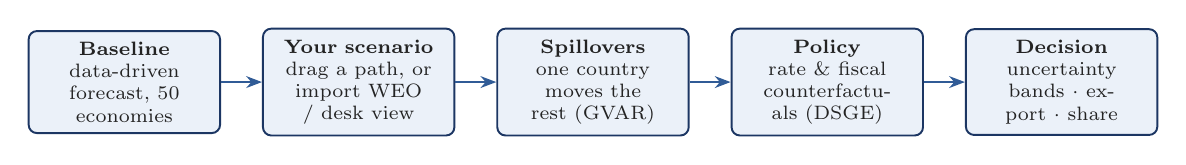
\begin{tikzpicture}
  \node[stage] (b) {\textbf{Baseline}\\ data-driven forecast, 50 economies};
  \node[stage, right=0.52cm of b] (s) {\textbf{Your scenario}\\ drag a path, or import WEO / desk view};
  \node[stage, right=0.52cm of s] (g) {\textbf{Spillovers}\\ one country moves the rest (GVAR)};
  \node[stage, right=0.52cm of g] (p) {\textbf{Policy}\\ rate \& fiscal counterfactuals (DSGE)};
  \node[stage, right=0.52cm of p] (d) {\textbf{Decision}\\ uncertainty bands $\cdot$ export $\cdot$ share};
  \draw[flowarr] (b) -- (s); \draw[flowarr] (s) -- (g); \draw[flowarr] (g) -- (p); \draw[flowarr] (p) -- (d);
\end{tikzpicture}
\end{center}
\vspace{0.1em}
\begin{columns}[T,onlytextwidth]
\begin{column}{0.52\textwidth}
  {\small\bfseries\color{MadridBlue} Why it matters}
  \begin{itemize}\setlength\itemsep{2pt}\small
    \plus \key{Speed} --- a coherent global ``what-if'' in an afternoon, not a forecasting round.
    \plus \key{Coherence} --- every number is mutually consistent, at home \emph{and} across borders.
    \plus \key{Reuse} --- folds in the forecasts we already produce (WEO, SPF, desk).
  \end{itemize}
\end{column}
\begin{column}{0.46\textwidth}
  {\small\bfseries\color{MadridBlue} What you can ask it}
  \begin{itemize}\setlength\itemsep{2pt}\small
    \item If US growth surprises --- who else moves, and by how much?
    \item If the Fed holds rates higher for longer, what happens here?
    \item If we take the WEO as given, what does it imply for everything else?
  \end{itemize}
\end{column}
\end{columns}
\end{frame}

% =============================================================================
% SECTION 1 - a: THE UNCONDITIONAL FORECAST
% =============================================================================
\begin{frame}{\textcircled{1}\; Start with the baseline --- no inputs, the model's own read of every economy}
\roadmap{1}
\vspace{0.2em}
{\small\centering \key{No assumptions required.} Each economy is a Bayesian VAR, linked into one global system.\par}
\vspace{0.3em}
\begin{center}
  \figmask{0.94\linewidth}{s1_macro_triad}\par\vspace{0.25em}
  {\footnotesize\color{Muted} US inflation, policy rate and GDP --- one consistent forecast, with uncertainty bands.}
\end{center}
\takeaway{The baseline}{A ready-made, internally consistent forecast for all \key{50 economies} --- the common starting point every scenario departs from.}
\end{frame}

% =============================================================================
% SECTION 1 - b: FISCAL ACCOUNTING -> DEBT/GDP
% =============================================================================
\begin{frame}{\textcircled{1}\; Fiscal accounting, built in --- the debt path drops out of the same run}
\roadmap{1}
\vspace{0.3em}
\begin{columns}[T,onlytextwidth]
\begin{column}{0.44\textwidth}
  \vspace{1.2em}
  {\small Revenue, spending, the interest bill and the deficit are projected \key{together} --- and debt-to-GDP follows from the \key{budget identity}.}
  \vspace{0.6em}

  {\small No separate spreadsheet: the fiscal story is \key{consistent with the macro forecast by construction}.}
\end{column}
\begin{column}{0.54\textwidth}
  \begin{center}
    \figmask{0.86\linewidth}{s1_debt_gdp}\par\vspace{0.25em}
    {\footnotesize\color{Muted} US debt-to-GDP rises to $\sim$143\% by 2031, with band.}
  \end{center}
\end{column}
\end{columns}
\takeaway{Why it matters}{Debt sustainability drops out of the \emph{same} run --- the macro and fiscal stories can never contradict each other.}
\end{frame}

% =============================================================================
% SECTION 2 - a: CONDITIONING — the everyday power move (credit crunch)
% =============================================================================
\begin{frame}{\textcircled{2}\; Tell it two things you believe --- it works out the rest, consistently}
\roadmap{2}
\vspace{0.3em}
\begin{columns}[T,onlytextwidth]
\begin{column}{0.42\textwidth}
  \vspace{1.0em}
  {\small\bfseries\color{MadridBlue} Recipe $\cdot$ Credit crunch}\par
  \begin{itemize}\setlength\itemsep{4pt}\small
    \item[\textcolor{MadridBlue}{\textbf{1.}}] Pin \key{spreads jump}.
    \item[\textcolor{MadridBlue}{\textbf{2.}}] Pin \key{lending falls}.
  \end{itemize}
  \vspace{0.4em}
  {\small Two pins in; the model works out a \key{full, coherent response} across every variable.}
\end{column}
\begin{column}{0.56\textwidth}
  \begin{center}
    \figmask{0.92\linewidth}{fig_credit_macro}\par\vspace{0.3em}
    {\footnotesize\color{Muted} US GDP response to the two credit pins, with bands.}
  \end{center}
\end{column}
\end{columns}
\takeaway{The power move}{A couple of believable pins $\rightarrow$ a full, consistent macro response --- a structural shock, no econometrics.}
\end{frame}

% =============================================================================
% SECTION 2 - b: A RICHER STORY NEEDS MORE PINS (energy supply shock)
% =============================================================================
\begin{frame}{\textcircled{2}\; A richer story? Just add a few more pins --- an energy shock}
\roadmap{2}
\vspace{0.3em}
\begin{columns}[T,onlytextwidth]
\begin{column}{0.49\textwidth}
  \begin{center}
    {\bfseries\color{MadridBlue} You pin}\par\vspace{0.3em}
    \figmask{0.76\linewidth}{fig_energy_oil}\par\vspace{0.25em}
    {\footnotesize\color{Muted} An oil-price path --- the size and shape of the spike.}
  \end{center}
\end{column}
\begin{column}{0.49\textwidth}
  \begin{center}
    {\bfseries\color{MadridBlue} Out comes}\par\vspace{0.3em}
    \figmask{0.76\linewidth}{fig_energy_macro}\par\vspace{0.25em}
    {\footnotesize\color{Muted} US stagflation: \key{prices up, output down}.}
  \end{center}
\end{column}
\end{columns}
\vspace{0.4em}
\takeaway{Fit the pins to the story}{The richer the story, the more you say up front --- an oil path plus a few transmission pins, and the same move does the rest.}
\end{frame}

% =============================================================================
% SECTION 3: THE GLOBAL SOLVE -- PARTNER TRANSMISSION (the killer slide)
% A global energy shock; ask a country-only model of the euro area -> it sees NOTHING;
% the coupled global solve reveals euro-area growth dragged to -0.8pp below baseline.
% =============================================================================
\begin{frame}{\textcircled{3}\; A shock abroad, a hit at home --- the part a country-only read cannot see}
\roadmap{3}
\vspace{0.5em}
\begin{columns}[T,onlytextwidth]
\begin{column}{0.49\textwidth}
  \begin{center}
    {\bfseries\color{Muted} Country-only read}\par\vspace{0.4em}
    \figmask{0.82\linewidth}{fig_partner_energy_dev_direct}\par\vspace{0.35em}
    {\footnotesize\color{Muted} Euro-area GDP vs baseline: \key{flat}.}
  \end{center}
\end{column}
\begin{column}{0.49\textwidth}
  \begin{center}
    {\bfseries\color{MadridBlue} Global solve}\par\vspace{0.4em}
    \figmask{0.82\linewidth}{fig_partner_energy_dev_coupled}\par\vspace{0.35em}
    {\footnotesize\color{Muted} The same shock arrives: \key{$-0.8$pp} by 2031.}
  \end{center}
\end{column}
\end{columns}
\vspace{0.7em}
\takeaway{Why the tool earns its keep}{A country-only read --- like the \gap{old GMF} --- shows \key{zero}; only the coupled solve reveals the hit.}
\end{frame}

% =============================================================================
% SECTION 4 - a: LONG-RUN ANCHORS
% =============================================================================
\begin{frame}{\textcircled{4}\; Pin the destination --- and the whole path tilts toward it}
\roadmap{4}
\vspace{0.3em}
\begin{columns}[T,onlytextwidth]
\begin{column}{0.44\textwidth}
  \vspace{1.0em}
  {\small Know only \key{where things should end up} --- the inflation target, potential growth, the neutral rate?}
  \vspace{0.6em}

  {\small Set that \key{long-run anchor}; the model tilts the path toward it, gently, \key{without breaking the near term}.}
\end{column}
\begin{column}{0.54\textwidth}
  \begin{center}
    \figmask{0.9\linewidth}{fig_ext_anchor}\par\vspace{0.3em}
    {\footnotesize\color{Muted} US inflation: the tail lands on the anchor (dashed); near term untouched.}
  \end{center}
\end{column}
\end{columns}
\takeaway{Long-run anchors}{Set where a variable \key{settles}; the path re-shapes to reach it, near term intact.}
\end{frame}

% =============================================================================
% SECTION 4 - b: EXTERNAL FORECASTS
% =============================================================================
\begin{frame}{\textcircled{4}\; Fold in an outside forecast as an ingredient --- at a trust level you choose}
\roadmap{4}
\vspace{0.3em}
\begin{columns}[T,onlytextwidth]
\begin{column}{0.44\textwidth}
  \vspace{1.0em}
  {\small A WEO number, a consensus figure, a desk view? \key{Import it directly} --- as one more ingredient, not a hard override.}
  \vspace{0.6em}

  {\small You set the \key{trust dial}: from ``just a hint'' to ``pin it exactly''. Everything else stays \key{consistent} around it.}
\end{column}
\begin{column}{0.54\textwidth}
  \begin{center}
    \figmask{0.86\linewidth}{fig_ext_weo}\par\vspace{0.25em}
    {\footnotesize\color{Muted} US GDP: teal diamonds are the imported WEO path.}
  \end{center}
\end{column}
\end{columns}
\takeaway{External forecasts}{Reuse the WEO and desk forecasts we \emph{already} produce --- as inputs, at a \key{trust level you control}.}
\end{frame}

% =============================================================================
% SECTION 4 - c: STRUCTURAL POLICY SHOCKS  (MMB / DSGE)
% =============================================================================
\begin{frame}{\textcircled{4}\; Ask ``what if the central bank does X?'' --- a genuine policy counterfactual}
\roadmap{4}
\vspace{0.3em}
\begin{columns}[T,onlytextwidth]
\begin{column}{0.44\textwidth}
  \vspace{0.7em}
  {\small This tells you \key{what a policy choice does} --- a \key{structural} answer from a fully specified DSGE model.}
  \vspace{0.5em}

  {\small Layer a \key{policy shock} on any scenario; the model traces the \key{counterfactual path}.}
\end{column}
\begin{column}{0.54\textwidth}
  \begin{center}
    \figmask{0.8\linewidth}{fig_ext_mmb}\par\vspace{0.25em}
    {\footnotesize\color{Muted} US policy rate: counterfactual vs.\ baseline scenario.}
  \end{center}
\end{column}
\end{columns}
\takeaway{Policy counterfactuals}{From ``what will happen'' to ``\key{what should we do}'' --- a structural (MMB/DSGE) policy experiment.}
\todo{on the roadmap: deeper MMB library, cross-country WEO propagation, external-balance/NFA satellite}
\end{frame}

% =============================================================================
% SECTION 5: CONCLUSION / THE ASK
% =============================================================================
\begin{frame}{\textcircled{5} One tool now gives us a current, global, and shareable read on policy — we ask you to adopt it}
\roadmap{5}
\begin{columns}[T,onlytextwidth]
\begin{column}{0.5\textwidth}
\textbf{What we built, in three lines:}
\begin{itemize}\setlength\itemsep{3pt}\small
\plus \key{Current \& consistent} --- every economy sits on the same up-to-date vintage, so the numbers add up across desks
\plus \key{Genuinely global} --- shocks travel across 50 economies through trade and finance, not one country at a time
\plus \key{Our forecasts, built in} --- WEO and staff views enter as dials, and any run is one-click \key{shareable and reproducible}
\end{itemize}
\end{column}
\begin{column}{0.48\textwidth}
\textbf{The arc:} a live baseline $\rightarrow$ \key{condition} it on the story you care about $\rightarrow$ let it \key{propagate globally} $\rightarrow$ layer in \key{policy and external-balance} extensions.

\vspace{0.6em}
\textbf{The ask:}
\todo{MF/Jesper: endorse the tool, resource the last-mile hardening, and adopt it into the FSAP / Article IV workflow.}

\vspace{0.4em}
{\small It is \key{live today}, covering \key{50 economies} — ready to pilot on the next surveillance cycle.}
\end{column}
\end{columns}
\vspace{0.4em}
\takeaway{The one line}{One live, shareable tool turns scattered forecasts into a single consistent, global answer to ``what if?''.}
\end{frame}

\end{document}
